\documentclass{article}
\usepackage[margin=1.2in]{geometry}
\usepackage[utf8]{inputenc}
\usepackage[english]{babel}
\usepackage{enumitem}
\usepackage{graphicx}
\usepackage{parskip}

\usepackage[backend=biber,style=numeric,sorting=ynt]{biblatex}
\usepackage{hyperref}
\addbibresource{project-specification.bib}

\begin{document}
    \title{CS310 Project Specification:\\Creating a Code Execution Toolchain from Compilation to Emulating a Custom RISC Processor}
    \author{Ruben Saunders\\2231825}
    \date{November, 2024}

    \maketitle

    \section{Problem Statement}\label{sec:problem-statement}

    When learning about processors, assembly language, and high-level programming languages, numerous online resources can significantly enhance your understanding and practical skills.
    For example, the Little Man Computer ~\cite{lmc} emulator provides a simplified model of a computer, making it easier to grasp basic processor operations and assembly language concepts.
    Similarly, MARS ~\cite{mars-simulator} (the MIPS Assembler and Runtime Simulator) is a platform for practicing the MIPS assembly language, allowing users to write, simulate, and debug code in an intuitive environment.

    While there are numerous tools for these individual aspects, resources that explore the interaction between these stages are more limited.
    Beyond merely compiling programs on a computer and examining the generated assembly or object files, websites like GodBolt Compiler Explorer ~\cite{godbolt} provide a more interactive experience, allows users to input high-level code and view the corresponding assembly output from various compilers.
    However, comprehensive tools that cover the entire process -- from writing high-level language code to executing it on a processor within a single environment -- are scarce.
    Such a tool would allow users to visualise and understand the entire workflow, offering an educational platform that integrates compiling, assembly translation, and execution.
    This contrasts with existing systems that are often complex and geared towards professional use, posing a barrier for learners.

    This project aims to fill this gap by designing and implementing the entire process -- from compiling a high-level language to emulating machine code on a custom RISC processor -- in a single environment.
    The project will consist of the following three layers:

    \begin{enumerate}
        \item A compiler which translates source code in a custom high-level language to assembly code.
        \item An assembler that converts this assembly code into a machine code binary.
        \item A RISC processor emulator that executes the machine code.
    \end{enumerate}

    Along with a TUI application demonstrating how all three layers relate during execution, allowing the user to observe and interact with the translation and execution of the program.

    As stated above, the goal of this project is to serve as an educational tool, with a design that prioritises simplicity at every stage.
    Each individual stage serves as a resource for students interested in exploring CPU architecture, assembly programming, compiler design, and the execution of high-level languages.
    Furthermore, as the project covers the entire process in a single tool, it additionally serves as a practical tool for insight into the interaction of said layers to produce a complete pipeline from start to end of program execution.

    \section{Objectives}\label{sec:objectives}

    Each of the three layers have been expanded into further details and aims.

    \begin{enumerate}
        \item Designing a RISC processor and implementing an emulator for it.
        \begin{enumerate}
            \item RISC design: the processor will have a simplified yet powerful ISA, providing only essential instructions that cannot be omitted or substituted.
            \begin{enumerate}
                \item All instructions will operate on registers, with data moved in to/out of registers via \texttt{move} and \texttt{store}, respectively.
                \item The ISA will be split into instruction classes: data movement, arithmetic, logical, comparison, control flow (jumping and function calling), and other.
                \item Operands may take multiple forms to allow for more flexibility: immediate, register, register indirect, memory address.
                \item Instructions may have a conditional restriction; that is, it only executes if a condition is met.
            \end{enumerate}
            \item The processor will have a word size of 64 bits.
            \begin{enumerate}
                \item Registers will be 64-bit, and will not have a datatype.
                If required, an instruction will contain a flag to identify the datatype of a register.
                \item The processor will provide both special registers and general purpose registers.
            \end{enumerate}
            \item The processor will support both integer and floating-point arithmetic and comparison.
            \item The system call operation will be used to implement non-trivial operations to avoid additional complexities.
            \begin{enumerate}
                \item A syscall will be provided to print a character to \texttt{stdout}.
                \item A syscall will be provided to retrieve a character from \texttt{stdin}.
            \end{enumerate}
            \item \textit{Optional}: the processor will support a primitive interrupt system.
            \item \textit{Optional}: the emulator may accept program arguments which will be pushed as strings on to the stack.
            This is a solution to provide command-line arguments without building an OS or similar wrapper.
        \end{enumerate}

        \item Designing an assembly language and writing an assembler to output a binary for the above processor.

        The assembly acts as a more readable and usable middle-ground between the high-level language and binary code.
        As a middle ground, it is not the focus of this project and is arguably not necessary;
        hence, other than to fulfill the needs of being able to fully express the capabilities of the processor, no extra thoughts or considerations will be developed.
        \begin{enumerate}
            \item Each line of assembly will be a comment, label, directives, or instructions.
            \begin{enumerate}
                \item Comments start with a semicolon and are used to erase the rest of the line.
                \item Labels are identifiers followed by a colon that may be used as references to a memory address, hence simplifying branching.
                \item Directives begin with a dot prefix, and are commands to the assembler, such as to reserve space, insert data, et cetera.
                \item Instructions begin with a mnemonic, followed by flags, then comma- or space-separated operands.
                \begin{enumerate}
                    \item Mnemonics will support overloading, with a signature translating to an opcode.
                    \item Each mnemonic's flags will be defined in the processor specification, but may include a conditional guard or datatype specifier.
                \end{enumerate}
            \end{enumerate}
        \end{enumerate}

        \item Designing a custom high-level language and writing a compiler to output the above assembly code.
        \begin{enumerate}
            \item The language will be imperative with a C-like structure.
            \begin{enumerate}
                \item Variables may be created on the stack with a given type which cannot change.
                \item Functions may be defined, with their signature consisting of its name and argument types.
                \item Functions may be overloaded.
                \item Data structures contain name--type fields, similar to structs in C.
                \textit{Optional}: data structures may contain methods.
                \item The language will support the following datatypes: signed and unsigned 32-- and 64-bit integers, floats, and doubles.
                \textit{Optional}: due to the flexibility of the stack, it will also support 8-- and 16-bit integers.
                \item Namespaces will be implemented to allow for name separation and modularisation.
                \item \textit{Optional}: Operators are functions, and may be overloaded.
            \end{enumerate}
            \item The program has the following stages:
            \begin{enumerate}
                \item Pre-processing: prior to lexing, directives prefixed with `\texttt{\%}' are handled.
                Examples include \texttt{\%include} to include additional files, and \textit{optionally}, \texttt{\%macro} to define a macro, \texttt{\%define} to define constants.
                \item Lexing: scan the source and transform into tokens.
                \item Parsing: from tokens, produce a syntax tree.
                \item Compilation: compile syntax tree into assembly code.
                Not all functions will be implemented at this stage; add declared but undefined symbols to a symbol table.
                \item Linking: using symbol tables from other compilation units, resolve undefined references.
                \item Loading: load all assembled units into one large assembly program.
            \end{enumerate}
            Hence, the compiler takes multiple input files and produces one assembly.
            \item The compiled output accepts command-line arguments as strings, with an entry point of \texttt{main}, taking either no arguments or the number of arguments and a pointer to an array of strings.
        \end{enumerate}

        \item Writing a TUI application to visualise the execution of a program across all three layers.
        \begin{enumerate}
            \item The user will have three views: the high-level code, the assembly, and the machine code (reconstructed assembly).
            \item Working backwards from the current machine code instruction, with corresponding lines/sections in both the assembly and high-level source code highlighted.
            \item Extra windows will be available for interactivity.
            \begin{enumerate}
                \item Register view/editor.
                \item Memory view/editor.
                \item Stack view/editor.
                View stack frames and label each value.
            \end{enumerate}
        \end{enumerate}
    \end{enumerate}

    \section{Methods \& Methodology}\label{sec:methods-&-methodology}

    The nature of the three sub-systems is that of developing a program to implement a standard, or specification, which appeals to plan-based methodologies.
    For example, the Waterfall model would ensure that all requisite documentation be fully complete prior to development.
    Implementation should not majorly impact the design and hence avoids a key disadvantage of plan-based approaches.

    Furthermore, from the perspective of the entire project, once documentation is complete, the next stage can commence even prior to implementation.
    This minimises the dependence between sub-systems, increasing design and development time on each, and allows for the project to be fully designing, reviewed, and adjusted prior to any implementation.

    This is additionally true for the TUI application which will combine the three, as it will mostly rely on previous documentation and completed work.
    However, development of features for observation and interaction will not have been documented fully prior to development, so this stage will take on more of an incremental approach.

    Kanban boards will be used to ensure tasks are completed and deadlines adhered to, and will serve as an indicator of progress.

    \section{Timetable}\label{sec:timetable}

    Each primary sub-system is designed to interface with the others to produce a fully functioning pipeline.
    However, implementation can proceed in any order, as long as the interfaces are well-documented and defined beforehand.
    Given this, documentation has been identified as the critical path because the interfaces and dependencies between sub-systems must be clearly defined before implementation can begin.

    The compiler has been identified to be the most complex sub-system, both in terms of design and implementation, so has been allotted more time.
    Additionally, due to the presence of the compiler design and principles of programming languages modules, this sub-system has the most to benefit from term-time.
    With that in mind, a preliminary plan has been created (figure~\ref{fig:gantt-chart}): the processor emulator and assembler are planned to be completed in term 1, with term 2 focusing on the compiler.

    The TUI application will be developed incrementally alongside each stage, but has been allotted time solely dedicated to it at the ends of term 1, as focus will be on developing the emulator and assembler, and in term 2, as the inclusion of the high-level language in the application is forseen to complicate development.
    This is because the relationship between machine code and assembler is generally one-to-one, compared to a high-level language.
    This complexity will be reduced be considering this hurdle and incorporating it into early design.

    \begin{figure}
        \centering
        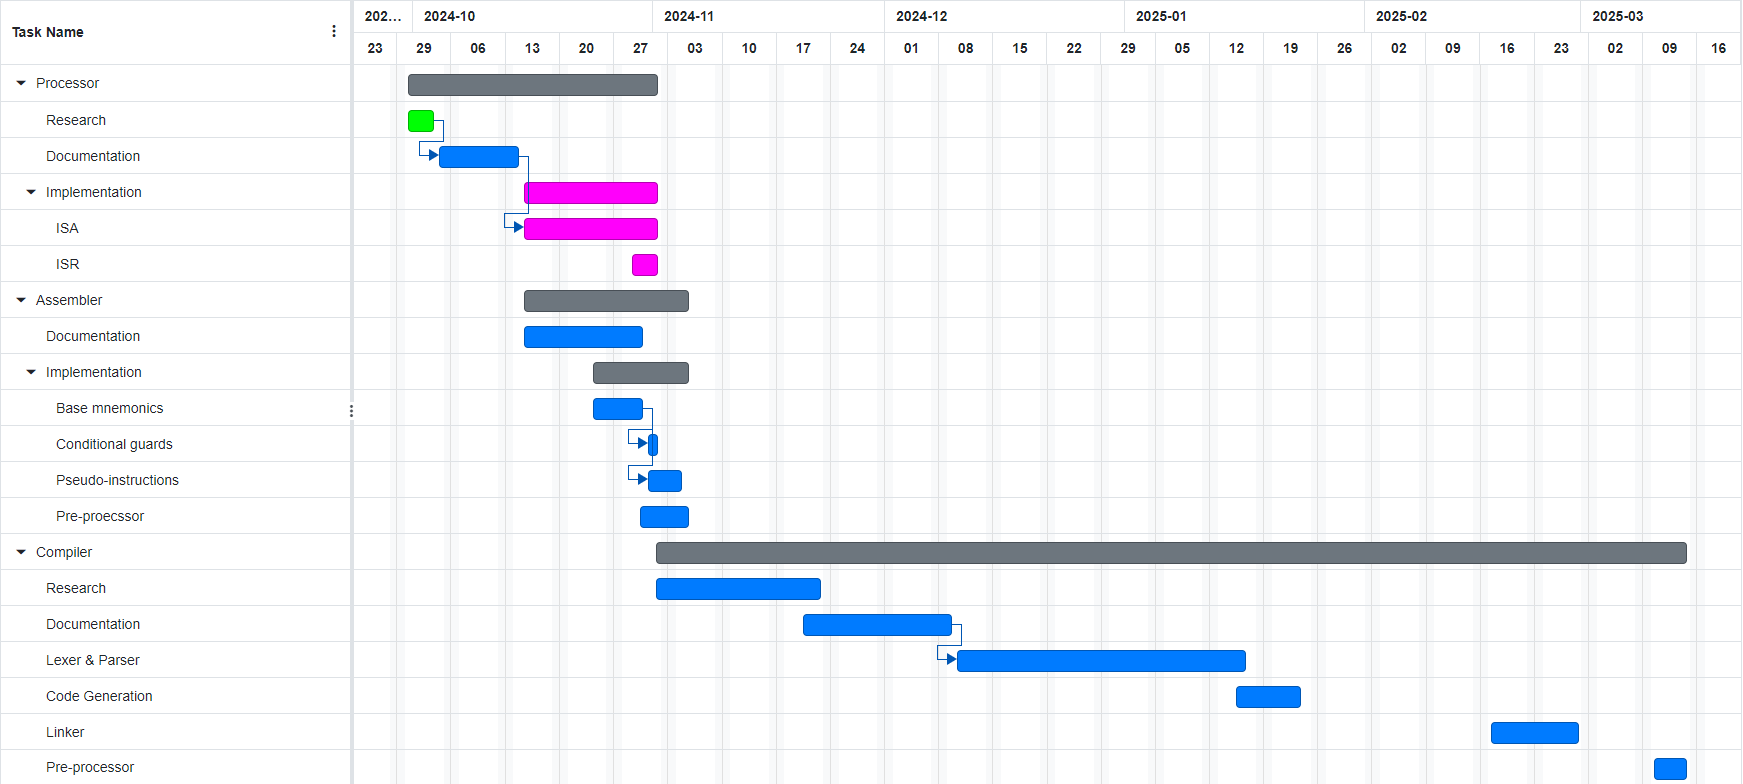
\includegraphics[width=\textwidth]{assets/project-gantt-chart}
        \caption{Preliminary project plan for term one}
        \label{fig:gantt-chart}
    \end{figure}

    Each sub-system's specification will be continually revised and validated against project objectives after each major revision.
    During implementation, it will act as a guide for progress, and any deviation or amendments will be documented and specification adjusted accordingly.

    \section{Technologies}\label{sec:technologies}

    The entire project will be tracked using \texttt{git} on \texttt{GitHub} under a single repository.
    Each sub-system will be located in a separate directory within the repository, allowing each to act as a stand-alone project while still being part of the overall system.

    The nature of the project requires a performant programming language, especially for the processor emulator.
    As this is an educational tool, the language should also be well-known and easy to understand.
    Hence, the shortlisted languages are \texttt{C}, \texttt{C++}, or \texttt{Rust}.

    All three languages are typically used in systems-level programming, are well-established, and documented.
    While \texttt{C} is flexible, it does not provide any native libraries for data structures or algorithms which may become useful in development, and would avoid external dependencies.
    Hence, due to its simplicity and lack of need for extra features and libraries, the processor emulator will be written in \texttt{C}, with the assembler and compiler written ion \texttt{C++}.

    Using a buildsystem, such as \texttt{makefile}, would be beneficial to the project in terms of file management and ease of compilation.
    As a further abstraction, \texttt{CMake} would further simplify the build process and dependency management.

    \section{Research}\label{sec:research}

    For processor research, the primary source will be the RISC-V architecture, which is a well-known and widely-adopted RISC processor.
    By first understanding the reasoning and defining features of RISC processors ~\cite{risc-vs-cisc}, this research will guide the design of the processor sub-system.
    The RISC-V documentation ~\cite{riscv-docs} will serve as a key resource for developing a sufficient instruction set and informing instruction layout and encoding.

    For further insights into instruction sets and assembly formats, the MIPS architecture will also be studied.
    MIPS is another RISC ISA, often used for educational purposes due to its simplicity and clarity.
    The MIPS instruction set architecture ~\cite{mips-isa} will provide additional context on required instructions, and further research will cover useful pseudo-instructions ~\cite{mips-pseudo-instructions}.

    Research for the high-level language and compiler sub-system has not yet been considered in detail.
    However, it is likely to involve reading the \texttt{C} documentation due to the language's history, simplistic nature, and familiarity with other existing languages.
    Additionally, both the Compiler Design and Principles of Programming Languages modules will serve as indispensable resources for this sub-system.

    \section{Legal, Social, Ethical \& Professional Considerations}\label{sec:considerations}

    The toolchain being developed is for educational purposes and will not be commercially released.
    Additionally, as each sub-system is custom designed, there are no copyright or licensing issues.
    Similarly, any libraries used will be \texttt{C++} standard libraries, so licenses are not an issue.

    As an educational tool which may require feedback or be used by minors, ethics must be considered.
    As such, appropriate safeguarding measures must be in place, including obtaining parental and University consent where necessary and ensuring that any feedback collected from minors is handled responsibly and in compliance with relevant privacy laws.

    This project does not require any social considerations.
    However, it is good practice and beneficial to students that the code be well-written and commented to be understandable, and any and all documentation should be readily available.

    \printbibliography
\end{document}